\documentclass[11]{article}

../../../../TexScripts/HeaderfileTexDocs.tex

\geometry{left=0.9in, right=0.9in, top=0.9in, bottom=0.9in}

\usepackage{Sweave}
\begin{document}
\Sconcordance{concordance:Project1_Report.tex:Project1_Report.Rnw:%
1 6 1 1 0 16 1 1 57 1 1 1 2 12 0 1 2 2 1 1 17 6 1 1 4 13 0 1 2 1 3 15 0 %
1 2 1 3 13 0 1 2 1 4 17 0 1 2 1 4 18 0 1 2 1 3 15 0 1 2 1 18 7 1 1 6 16 %
0 1 2 8 1 1 18 7 1 1 13 2 1 1 57 15 0 1 4 6 1}

%\SweaveOpts{width='3in',height='3in'}
\doublespacing

\title{Project 1: What influences self reporting of Concussion in undergraduate college students?}
\author{Subhrangshu Nandi, UW Madison Department of Statistics \\
Dr. Traci Snedden (PhD, RN, CPNP, CNE), UW Madison School of Nursing
}
%\date{March 13, 2014}
\maketitle
\subsubsection*{Purpose}
To investigate the factors that might influence ``self-reporting'' of {\bf{concussion}} and why it may occur, in undergraduate college students. 

\subsubsection*{Data}
The data is from a survey send out to a large groups of undergraduate students at a large midwestern university. Overall response rate of the survey was $6.72\%$ (1,950 out of 29,000). The response rate is slightly lower than the average response rate for external surveys which is around 10-15\%. Out of 1,950 respondents, 76 of them reported to have had a concussion during since starting college. We analyzed this subset to investigate the factors that might influence ``self-reporting'' of concussion and the reasons why they may have occurred. 

\subsubsection*{Summary}
Of the 76 students who had concussion, the only 31 ``self-reported'', as shown in table \ref{tab:tab1Summary}.
% latex table generated in R 3.3.1 by xtable 1.8-2 package
% Thu Apr  6 09:48:51 2017
\begin{table}[ht]
\centering
\begin{tabular}{rrr}
  \hline
NA & YES & NO \\ 
  \hline
  8 &  31 &  37 \\ 
   \hline
\end{tabular}
\caption{Self-reporting of concussion} 
\label{tab:tab1Summary}
\end{table}
The plot (fig \ref{fig:Fig1Age}) below shows the distribution of ages of students in the three sub-groups - "YES", "NO" and Missing information

\begin{figure}[H]
\centering
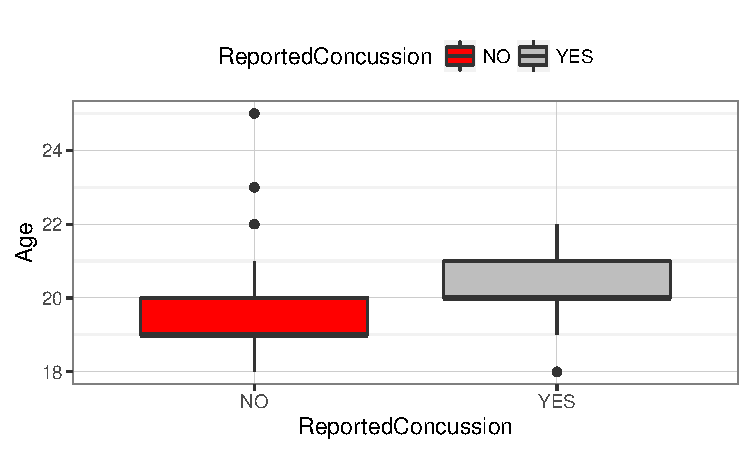
\includegraphics[width=0.5\linewidth]{Plot1Age.pdf}
\caption{Distribution of Age of students who had concussion, separated by whether they self-reported or not}
\label{fig:Fig1Age}
\end{figure}
Figure \ref{fig:Fig1Age} excludes one student whose age was 37 in the "YES" category. Apart from the three outlier points, students who did not self-report seem younger than the groups of students who did report. Table \ref{tab:Tab2Gender} shows the distribution of self-reporting behavior by gender. 
% latex table generated in R 3.3.1 by xtable 1.8-2 package
% Thu Apr  6 09:48:52 2017
\begin{table}[H]
\centering
\begin{tabular}{lrrr}
  \hline
 & NA & YES & NO \\ 
  \hline
Female &   5 &  25 &  25 \\ 
  Male &   3 &   6 &  12 \\ 
   \hline
\end{tabular}
\caption{Self-reporting of concussion} 
\label{tab:Tab2Gender}
\end{table}A $\chi^2$ test was conducted to test the hypothesis that self-reporting behavior was the same for both gender. Although the number of male students who did not self-report were twice that of female students, the difference in the distributions were statistically not significant. The p-value of the $\chi^2$ test was $0.3465$. Hence, we could not reject the null hypothesis. Below is the distrution of self-reporting behavior by ``race''.
% latex table generated in R 3.3.1 by xtable 1.8-2 package
% Thu Apr  6 09:48:52 2017
\begin{table}[H]
\centering
\begin{tabular}{lrrr}
  \hline
 & NA & YES & NO \\ 
  \hline
Asian &   3 &   0 &   3 \\ 
  Black or African American &   0 &   0 &   1 \\ 
  Others &   2 &   0 &   2 \\ 
  White &   3 &  27 &  31 \\ 
   \hline
\end{tabular}
\caption{Self-reporting of concussion by Race} 
\label{tab:Tab3Race}
\end{table}There were not enough students in all the cells of table \ref{tab:Tab3Race} to conduct a statistical test. There were also not enough students in all cells of ``ethnicity'' in table \ref{tab:Tab4Eth}
% latex table generated in R 3.3.1 by xtable 1.8-2 package
% Thu Apr  6 09:48:52 2017
\begin{table}[H]
\centering
\begin{tabular}{lrrr}
  \hline
 & NA & YES & NO \\ 
  \hline
Hispanic or Latino or Spanish Origin &   0 &   2 &   1 \\ 
  Not Hispanic or Latino or Spanish Origin &   6 &  28 &  36 \\ 
   \hline
\end{tabular}
\caption{Self-reporting of concussion by Ethnicity} 
\label{tab:Tab4Eth}
\end{table}Table \ref{tab:Tab5Acad} below is the distribution of self-reporting behavior by academic status.
% latex table generated in R 3.3.1 by xtable 1.8-2 package
% Thu Apr  6 09:48:52 2017
\begin{table}[H]
\centering
\begin{tabular}{lrrr}
  \hline
 & NA & YES & NO \\ 
  \hline
NA &   1 &   0 &   0 \\ 
  Completed 1 year or less &   1 &   5 &  10 \\ 
  Completed 1-2 years &   1 &   3 &   9 \\ 
  Completed 2-3 years &   4 &  14 &   8 \\ 
  Completed 3-4 years &   1 &   8 &   6 \\ 
  Completed 4 years or more &   0 &   1 &   4 \\ 
   \hline
\end{tabular}
\caption{Self-reporting of concussion by Academic status} 
\label{tab:Tab5Acad}
\end{table}Table \ref{tab:Tab6Desc} displays the type of physical activities the students were involved in. 
% latex table generated in R 3.3.1 by xtable 1.8-2 package
% Thu Apr  6 09:48:52 2017
\begin{table}[H]
\centering
\begin{tabular}{lrrr}
  \hline
 & NA & YES & NO \\ 
  \hline
NA &   0 &   0 &   1 \\ 
  NCAA-sanctioned D1 athlete &   0 &   0 &   2 \\ 
  Club sport at UW-Madison &   0 &   2 &   4 \\ 
  Intramural activities/sports at UW-Madison &   1 &   7 &  10 \\ 
  Uses UW-Madison physical activity/exercise facilities &   4 &  15 &  15 \\ 
  Does not participate in any activities &   2 &   6 &   4 \\ 
  Others &   1 &   1 &   1 \\ 
   \hline
\end{tabular}
\caption{Self-reporting of concussion by type of activity} 
\label{tab:Tab6Desc}
\end{table}In both, tables \ref{tab:Tab5Acad} and  \ref{tab:Tab6Desc}, there was not enough representation in all the cells to conduct statistical hypothesis testing. Table \ref{tab:Tab7Reason} displays the summary when asked if this was an athletic injury that occurred playing any level of UW sport (NCAA sanctioned D1, UW Club or UW RecSports/Intramurals) \\
% latex table generated in R 3.3.1 by xtable 1.8-2 package
% Thu Apr  6 09:48:52 2017
\begin{table}[H]
\centering
\begin{tabular}{lrrr}
  \hline
 & NA & YES & NO \\ 
  \hline
No &   3 &  27 &  32 \\ 
  Yes, NCAA-sanctioned D1 &   0 &   0 &   2 \\ 
  Yes, UW Club &   0 &   1 &   0 \\ 
  Yes, UW RecSports/Intramurals &   0 &   3 &   3 \\ 
   \hline
\end{tabular}
\caption{Self-reporting of concussion by reason} 
\label{tab:Tab7Reason}
\end{table}Only 9 out of 76 students reported that the injury had occurred playing some level of UW sport. When asked the number of hours after the injury occurred when they reported, following are the distributions by gender for those who reported within 4 days. In addition to these students, there were two students who reported after one week (7 days) and one student after two weeks. These were excluded from the boxplot in figure \ref{fig:Fig3HoursGender} to better illustrate the distribution of the rest of the students.
\begin{figure}[H]
\centering
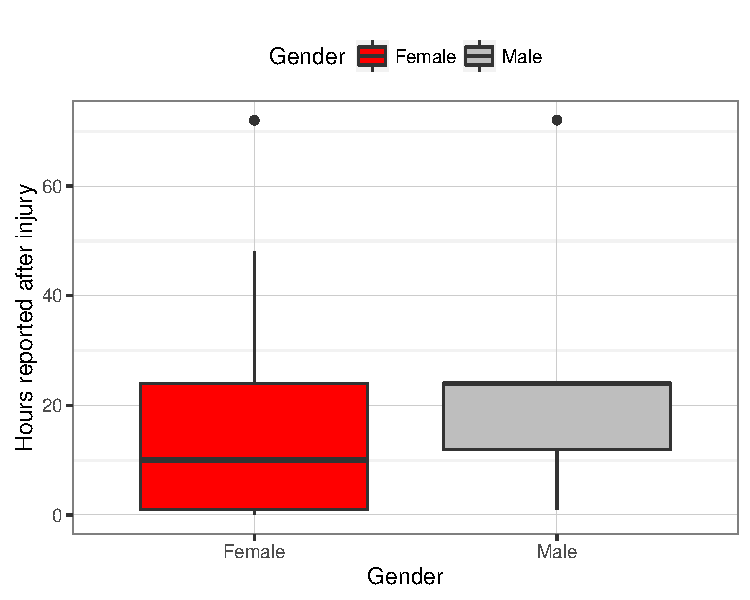
\includegraphics[width=0.5\linewidth]{Plot2ReportHours.pdf}
\caption{Distribution of Hours reported after injury, by Gender}
\label{fig:Fig3HoursGender}
\end{figure}

Of the students who self-reported, when asked who they reported to, only 6 students reported to ``parents'' and 6 students reported to ``others''. Of the students who did not self-report, following are the reasons whey behind their not reporting.
% latex table generated in R 3.3.1 by xtable 1.8-2 package
% Thu Apr  6 09:48:53 2017
\begin{table}[H]
\centering
\begin{tabular}{l|r}
  \hline
 & responses \\ 
  \hline
Didn’t know who to report it to &   2 \\ 
  Didn’t realize seriousness &   9 \\ 
  Didn’t think it was an injury &   6 \\ 
  Didn’t want to miss school &   1 \\ 
  Other (specify) &   5 \\ 
   \hline
\end{tabular}
\caption{Why did they not report} 
\label{tab:Tab8WhyNot}
\end{table}
\subsubsection*{Statistical Model}
Of all the factors, Age and Gender (although not statistically significant), showed some difference in self-reporting behavior. Below is a plot which illustrates the possible interaction between Age and Gender. Older females and younger males seem to have self-reported. We build a model to predict the odds of self-reporting, from the student's age and gender. We fit a logistic regression model:
\begin{equation}
Y = \beta_0 + \beta_1 X + \beta_2 G
\label{eq:Eq1}
\end{equation}
where, $Y = 1$, if self-reported, otherwise, $Y=0$, $X$ is the age of the student and $G$ is the gender. 


\begin{figure}[H]
\centering
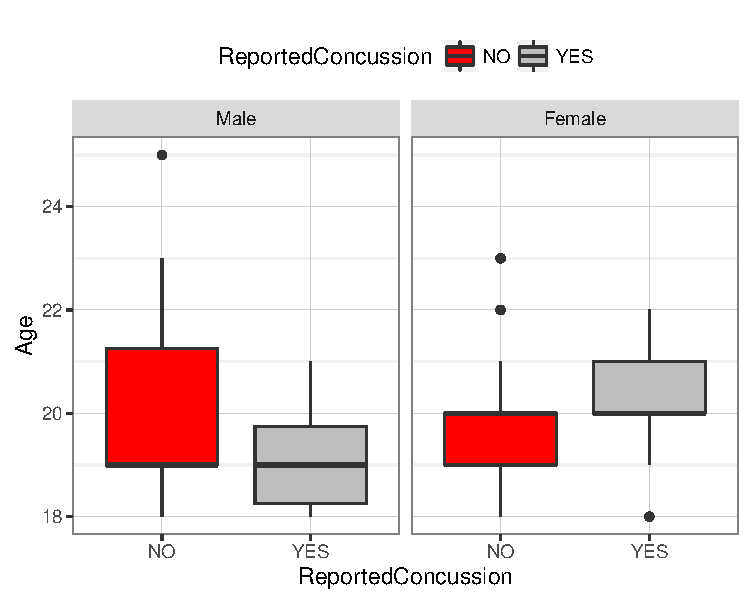
\includegraphics[width=0.5\linewidth]{Plot3AgeGender.pdf}
\caption{Distribution of Age, by Gender and self-reporting behavior}
\label{fig:Fig3AgeGender}
\end{figure}


Logistic regression was used to estimate the probability of self-reporting. Two predictor variables - age of student and gender of student, were used in the analysis, with simultaneous entry of predictors. As shown in table \ref{tab:Tab8}, the overall predictive model was statistically significant (likelihood ratio chi-square = 10.15 [4], p < 0.05). The independent variables age and the interaction of age with gender were both significant in predicting the likelihood of self-reporting. On an average, older students were more likely to self-report. Females, on an average, were more likely to self-report. However, older males were less likely to self-report (OR = -2.19). Although the overall model and the two predictors were statistically significant, the classification results indicated modest success, with an overall rate of correct classification of 64.71\%. The overall effect size was also modest, with the Nagelkerke R$^2$ equal to 10.83\%.

% latex table generated in R 3.3.1 by xtable 1.8-2 package
% Thu Apr  6 09:48:54 2017
\begin{table}[H]
\centering
\begin{tabular}{lrrrrr}
  \hline
Predictor & b(SE) & Wald & Odds Ratio & Lower OR & Upper OR \\ 
  \hline
Constant & 0.09 (0.31) & 0.28 & 1.09 & 0.6 & 2.02 \\ 
  Age & 0.66 (0.3) & 2.23* & 1.93 & 1.14 & 3.68 \\ 
  Male & -1.01 (0.68) & -1.49 & 0.36 & 0.07 & 1.24 \\ 
  Age:Male & -1.03 (0.47) & -2.19* & 0.36 & 0.12 & 0.81 \\ 
   \hline
\end{tabular}
\caption{Logistic Regression Results Predicting the Probability of Self Reporting} 
\label{tab:Tab8}
\end{table}
The coefficient of age was 0.659 (p < 0.05), which implied that with age the log odds of reporting increased, i.e., for every one year of age, the odds of self-reporting increased by 1.933 (which was $e^{0.659}$). For males, the odds of self-reporting was 0.363 (log odds = -1.012) compared to females, although the p-value was large. This was possibly due to the imbalance in the data (50 females vs 18 males). The interaction term between age and gender was -1.03 (p-value < 0.05), which implied that for males, the odds of self reporting reduces by 0.356 for every one year of age. This was consistent with the pattern in figure \ref{fig:Fig3AgeGender}. The prediction model can be used for prediction: the probability of a 18 year old female to self-report was 20\%, and male was 47\%. But for a 22 year old female it was 78\%, but male was 17\%. 

\subsubsection*{Limitations}
The summary and statistical findings, although interesting, have some limitations. The sample size was 76, and out of them 8 students did not respond to the question on self-reporting, further reducing the sample size to 68 students. Further analysis is necessary to assert if these non-respondents could be asserted as "missing-at-random". More respondents with information like the reason for injury, their activities, etc, would improve the predictive power of this model. A more balanced sample, in terms of the predictors would improve the robustness of the results. For example, if more males responded to the survey it would improved the gender balance. 

\end{document}
